\chuong{MÔ TẢ VÀ PHÂN TÍCH DỮ LIỆU BÁN HÀNG}

\subsection{Tổng quan về Adventure Works Cycles}

Adventure Works Cycles là một doanh nghiệp hư cấu do Microsoft dựng nên làm bối cảnh cho bộ cơ sở dữ liệu mẫu AdventureWorks và các bài hướng dẫn về công cụ phân tích của hãng. Theo mô tả của Microsoft, đây là một công ty sản xuất đa quốc gia quy mô lớn, chế tạo và phân phối xe đạp khung kim loại lẫn vật liệu composite cho các thị trường thương mại ở Bắc Mỹ, châu Âu và châu Á \citep{microsoft-scenario}. Trụ sở đặt tại Bothell, bang Washington, nơi công ty sử dụng 500 lao động, và đi kèm là nhiều nhóm bán hàng khu vực phân bố khắp địa bàn kinh doanh \citep{microsoft-scenario}.

Ở khâu sản xuất, công ty từng mua lại một cơ sở nhỏ tại Mexico là Importadores Neptuno, chuyên làm các linh kiện quan trọng rồi chuyển về Bothell để lắp ráp thành phẩm. Sau một năm tài chính thuận lợi, ban lãnh đạo muốn mở rộng thị phần theo ba hướng: nhắm quảng cáo vào nhóm khách hàng tốt nhất, mở rộng khả năng tiếp cận sản phẩm qua một website bên ngoài, và giảm chi phí bán hàng bằng cách hạ chi phí sản xuất. Cả ba hướng đều cần phân tích doanh số theo khách hàng, kênh bán và sản phẩm. Đó cũng là lý do hoạt động bán hàng được chọn làm trọng tâm của đồ án này.

Adventure Works Cycles phù hợp với đề tài là do chính Microsoft đã mô tả một môi trường phân tích tương tự. Trong kịch bản của hãng, dữ liệu giao dịch từ cơ sở dữ liệu AdventureWorks2012 được kết hợp với các thông tin phi giao dịch như chỉ tiêu doanh số lấy từ bảng tính, rồi hợp nhất vào kho dữ liệu AdventureWorksDW2019. Nhóm phụ trách kho dữ liệu của công ty đánh giá kho này là cơ sở dữ liệu chiều được thiết kế tốt, có chiều dùng chung và khóa thay thế. Nhờ vậy, bộ dữ liệu vừa cho ta nguồn giao dịch để xử lý, vừa cho một mô hình chiều hoàn chỉnh để đối chiếu khi thiết kế kho trên Microsoft Fabric~\citep{microsoft-scenario}.

\subsection{Tổng quan hoạt động bán hàng}
\subsubsection{Quy trình bán hàng}
Trong dữ liệu nguồn, một đơn hàng gồm bản ghi đầu đơn tại \texttt{Sales.SalesOrderHeader} và các dòng hàng tại \texttt{Sales.SalesOrderDetail}. Đầu đơn lưu ngày đặt hàng, khách hàng, khu vực, kênh đặt hàng và trạng thái; dòng hàng lưu sản phẩm, số lượng, đơn giá và chiết khấu. Quan hệ này cho phép đi từ giao dịch phát sinh đến số đo doanh thu ở mức từng sản phẩm trong đơn~\citep{aw-samples}.
\subsubsection{Các đối tượng tham gia hoạt động bán hàng}
Các đối tượng chính trong phạm vi phân tích là đơn hàng, sản phẩm, khách hàng và lãnh thổ bán hàng. Dữ liệu sản phẩm nối tiếp tới phân nhóm và danh mục; khách hàng có thể gắn với cá nhân hoặc cửa hàng. Những quan hệ này được mô tả trong script nguồn \texttt{AdventureWorks/raw/instawdb.sql} và sơ đồ ở Hình~\ref{fig:aw-oltp-schema}.
\subsubsection{Các chỉ tiêu đánh giá hoạt động bán hàng}
Các chỉ tiêu dự kiến gồm doanh thu dòng hàng, số lượng sản phẩm bán và số đơn hàng. \texttt{LineTotal} của dòng hàng được định nghĩa từ đơn giá, tỷ lệ chiết khấu và số lượng; \texttt{TotalDue} ở đầu đơn gồm tạm tính, thuế và phí vận chuyển. Khi so sánh hai mức số đo phải nêu rõ có cộng thuế và phí vận chuyển hay không~\citep{aw-samples}.
\subsection{Nguồn gốc và cấu trúc dữ liệu}
\subsubsection{Nguồn dữ liệu Adventure Works}

Bộ AdventureWorks do Microsoft công bố ban đầu để minh họa cách thiết kế cơ sở dữ liệu trên SQL Server 2008. Trong đó, AdventureWorks là mẫu xử lý giao dịch trực tuyến (OLTP), còn AdventureWorksDW là mẫu kho dữ liệu. Về sau Microsoft tiếp tục phát hành phiên bản mới theo từng đời SQL Server, hiện trải từ 2008 R2 đến 2025, và chia thành ba biến thể: OLTP cho các khối lượng công việc giao dịch thông thường, DW cho kho dữ liệu, và LT là bản gọn nhẹ rút ra từ OLTP~\citep{aw-samples}.

Đồ án lấy bộ dữ liệu thô OLTP làm đại diện cho nguồn dữ liệu, với bộ script và tệp dữ liệu được lấy từ kho mã nguồn sql-server-samples của Microsoft trên GitHub. Nhóm có lựa chọn này xuất phát từ bản chất của dữ liệu OLTP, vì đây là dữ liệu phát sinh trực tiếp từ vận hành, chưa được mô hình hóa cho mục đích phân tích, đúng với dạng đầu vào mà một kho dữ liệu trong thực tế phải tiếp nhận. Từ nguồn này, dữ liệu sẽ lần lượt đi qua quy trình Medallion chuẩn trên Microsoft Fabric để hình thành mô hình phục vụ phân tích. Bộ script kho dữ liệu cùng kho mã nguồn được dùng làm mô hình tham chiếu khi thiết kế lớp đích. Biến thể LT không được sử dụng vì đây chỉ là bản rút gọn của OLTP.

\subsubsection{Cấu trúc dữ liệu nguồn}

Nguồn dữ liệu OLTP mô hình hóa hoạt động của AdventureWorks Cycles theo hướng ghi nhận giao dịch, với lược đồ chuẩn hóa ở mức cao. Ở dạng này, mỗi loại thông tin được tách thành bảng riêng và liên kết với nhau qua khóa, nhằm hạn chế dư thừa và giữ tính nhất quán khi dữ liệu liên tục được ghi và sửa.

Toàn bộ cơ sở dữ liệu được chia thành năm lược đồ. Cách chia này bám theo các bộ phận chính của một doanh nghiệp sản xuất, nên dữ liệu về cùng một đối tượng thường nằm rải rác ở nhiều lược đồ, mỗi lược đồ ứng với một mảng nghiệp vụ được mô tả trong bảng dưới đây:

\begin{table}[htbp]\centering
\caption{Các lược đồ nghiệp vụ trong AdventureWorks OLTP}
\label{tab:aw-schemas}
\begin{tabularx}{\textwidth}{|l|X|}\hline
\textbf{Lược đồ} & \textbf{Vai trò} \\ \hline
HumanResources & Thông tin nhân sự \\ \hline
Person & Thông tin cá nhân, liên hệ và địa chỉ \\ \hline
Production & Sản phẩm và hoạt động sản xuất \\ \hline
Purchasing & Mua hàng và nhà cung cấp \\ \hline
Sales & Bán hàng và khách hàng \\ \hline
\end{tabularx}
\end{table}

Ngoài năm lược đồ trên còn có một số bảng hệ thống dùng để ghi nhận lỗi và lịch sử thay đổi cấu trúc cơ sở dữ liệu. Các bảng này nằm ở lược đồ dbo và không mang thông tin nghiệp vụ, nên nằm ngoài phạm vi khai thác của đồ án.

\begin{figure}[H]\centering
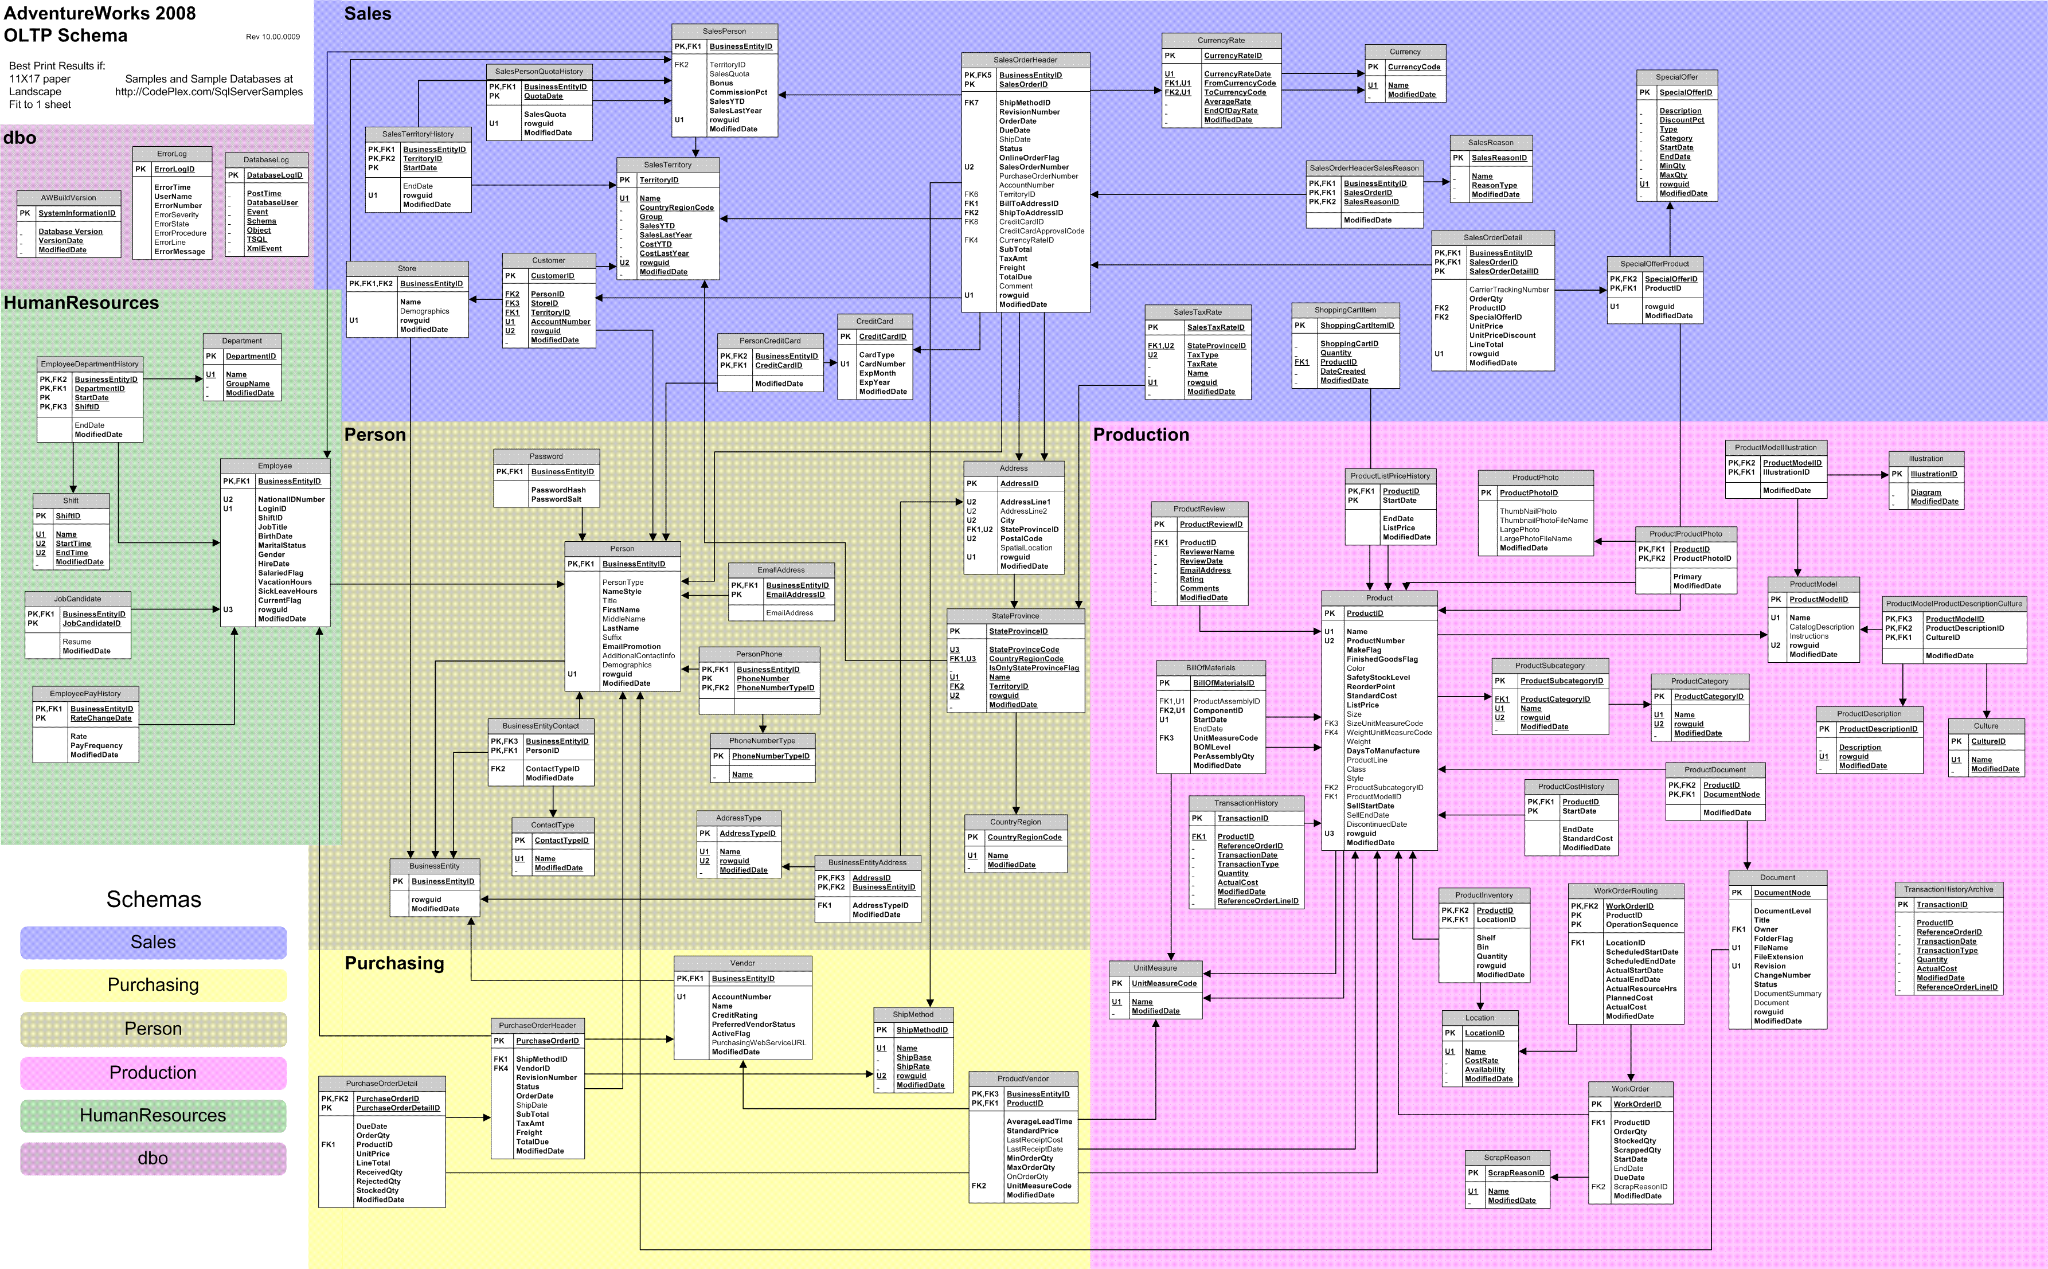
\includegraphics[width=\textwidth,height=0.6\textheight,keepaspectratio]{chapter-2/adventureworks-oltp-schema.png}
\caption{Sơ đồ tổng quát AdventureWorks OLTP 2008 (nguồn: \citealp{aw-schema}).}
\label{fig:aw-oltp-schema}
\end{figure}

Khác với OLTP, AdventureWorksDW được tổ chức theo mô hình chiều và gồm hai nhóm bảng. Nhóm thứ nhất là bảng sự kiện, có tiền tố Fact, chứa các số đo định lượng phát sinh từ nghiệp vụ. Nhóm thứ hai là bảng chiều, có tiền tố Dim, chứa các thông tin mô tả ngữ cảnh như khách hàng, sản phẩm, thời gian hay lãnh thổ. Các bảng liên kết với nhau bằng khóa thay thế có hậu tố Key, thay vì dùng trực tiếp mã nghiệp vụ của hệ thống nguồn.

Sự khác biệt giữa hai cách tổ chức này chính là lý do đồ án cần một quy trình chuyển đổi. OLTP được tối ưu cho việc ghi nhận giao dịch, còn mô hình chiều được tối ưu cho truy vấn và phân tích. Việc đưa dữ liệu từ nguồn thô đến mô hình chiều là nội dung của các chương sau.

\subsubsection{Các bảng dữ liệu phục vụ hoạt động bán hàng}
Nhóm bảng lõi gồm \texttt{SalesOrderHeader}, \texttt{SalesOrderDetail}, \texttt{Customer}, \texttt{SalesTerritory}, \texttt{Product}, \texttt{ProductSubcategory} và \texttt{ProductCategory}. Các bảng \texttt{Person} và \texttt{Store} bổ sung thông tin mô tả khách hàng. Khi triển khai cần kiểm tra khả năng nối từng bảng và cách xử lý khóa ngoại thiếu giá trị trước khi dùng làm chiều phân tích. Cấu trúc cột được đối chiếu từ \texttt{AdventureWorks/raw/instawdb.sql}~\citep{aw-samples}.
\subsubsection{Mối quan hệ giữa các bảng dữ liệu}
\texttt{SalesOrderDetail.SalesOrderID} nối với \texttt{SalesOrderHeader.SalesOrderID}; \texttt{ProductID} nối dòng hàng với sản phẩm. \texttt{CustomerID} và \texttt{TerritoryID} ở đầu đơn dẫn đến khách hàng và lãnh thổ. Từ sản phẩm có thể đi qua \texttt{ProductSubcategoryID} rồi \texttt{ProductCategoryID} để phân tích theo nhóm. Đây là đường nối dự kiến cho mô hình phân tích; số bản ghi mất liên kết cần được kiểm tra trên dữ liệu đã nạp.
\subsection{Khám phá và trực quan hóa dữ liệu}
\subsubsection{Phân tích doanh thu theo kênh bán hàng}
Cột \texttt{OnlineOrderFlag} ở đầu đơn có thể dùng để tách đơn đặt trực tuyến và đơn qua kênh khác. Bảng tổng hợp cần dùng cùng quy tắc trạng thái đơn và cùng định nghĩa doanh thu cho cả hai kênh.
\subsubsection{Phân tích doanh thu theo nhóm sản phẩm}
\texttt{ProductSubcategory} và \texttt{ProductCategory} cung cấp hai cấp phân nhóm. Khi tổng hợp, cần giữ cả sản phẩm chưa có phân nhóm để không làm mất doanh thu.
\subsubsection{Phân tích doanh thu theo thời gian}
\texttt{OrderDate} là mốc đặt hàng; \texttt{ShipDate} là mốc giao hàng và có thể trống. Nhóm sẽ chọn một ngày nghiệp vụ thống nhất trước khi tính chuỗi doanh thu theo tháng và năm.
\subsubsection{Phân tích khách hàng}
\texttt{CustomerID} cho phép đếm khách hàng phát sinh đơn. Việc phân loại cá nhân và cửa hàng dựa vào \texttt{PersonID} và \texttt{StoreID}; các trường hợp hai khóa cùng có giá trị cần được đối chiếu với định nghĩa trong dữ liệu nguồn.
\subsubsection{Phân tích doanh thu theo khu vực}
\texttt{TerritoryID} trên đầu đơn nối với \texttt{SalesTerritory}, nơi có tên lãnh thổ, quốc gia và nhóm khu vực. Doanh thu theo khu vực sẽ dùng lãnh thổ ghi tại thời điểm đơn hàng, tránh suy ngược từ địa chỉ hiện tại của khách hàng.
\subsection{Xác định yêu cầu dữ liệu cho giải pháp}
\subsubsection{Xác định quy trình nghiệp vụ}
Quy trình được chọn là bán hàng. Dữ liệu đầu đơn và dòng hàng là cơ sở để theo dõi doanh thu, số lượng bán và số đơn hàng theo các chiều phân tích.
\subsubsection{Xác định mức độ chi tiết dữ liệu}
Bảng sự kiện bán hàng dự kiến có một dòng cho mỗi \texttt{SalesOrderDetailID}. Mức chi tiết này giữ được liên hệ với sản phẩm, số lượng, giá và chiết khấu của từng dòng; các thuộc tính đầu đơn được đưa vào qua \texttt{SalesOrderID}.
\subsubsection{Xác định các chiều phân tích}
Những chiều tối thiểu gồm ngày đặt hàng, sản phẩm, khách hàng, lãnh thổ và kênh bán.
\subsubsection{Xác định các chỉ tiêu đo lường}
Các số đo tối thiểu gồm số lượng, doanh thu dòng hàng và số đơn hàng phân biệt. Thuế và phí vận chuyển ở mức đầu đơn sẽ được trình bày riêng để tránh cộng lặp khi một đơn có nhiều dòng.
\subsubsection{Xác định yêu cầu dữ liệu cho Machine Learning}
Bài toán dự báo doanh số cần chuỗi thời gian được tổng hợp ở một mức hạt và đơn vị tiền thống nhất. Tập huấn luyện và kiểm tra sẽ được tách theo thời gian; kết quả dự báo phải ghi rõ kỳ dự báo, dữ liệu lịch sử và sai số đánh giá trước khi đưa vào báo cáo.
